\section{MT-DNN-1}
\label{sec:mt-dnn-1}

\subsection{Preliminaries}
\label{subsec:prelim}
In this work, our multi-task model combines classification, regression and pair-wise ranking tasks, which are summerised in Table~\ref{tab:task}. We briefly introduce the definition of each task as follows: 
\begin{table}[htb!]
	\begin{center}
		\begin{tabular}{@{\hskip1pt}l@{\hskip1pt}|@{\hskip1pt}c@{\hskip1pt}|@{\hskip1pt}c@{\hskip1pt}|@{\hskip1pt}c}
			\hline \bf Input &Classification&Regression &Ranking\\ \hline \hline
			single sentence &$\checkmark$&& \\
			pairwise text &$\checkmark$&$\checkmark$&$\checkmark$ \\ \hline
		\end{tabular}
	\end{center}
	\lgspace
	\caption{Summary of tasks in our multi-task framework.
	}
	\label{tab:task}
\lgspace
\end{table}
\begin{figure}[!t]
\centering
\adjustbox{trim={.065\width} {.01\height} {.05\width} {.01\height},clip}
{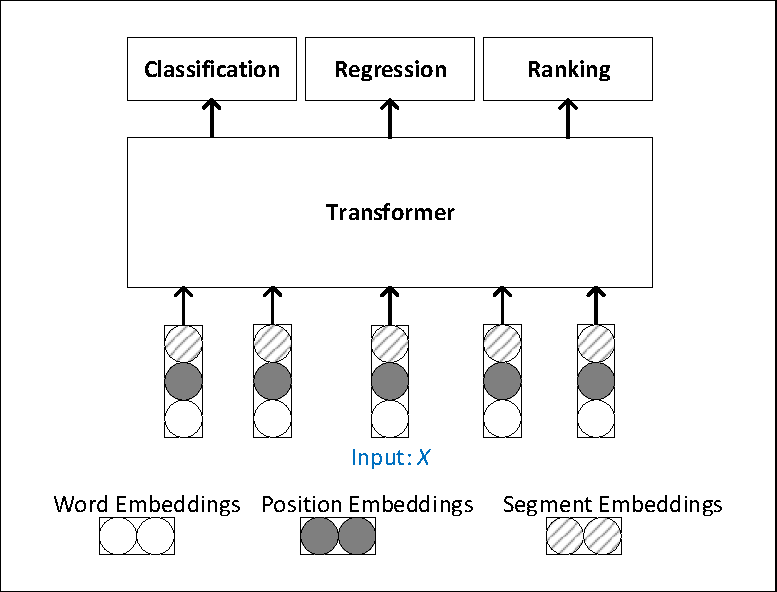
\includegraphics[scale=0.7]{mtl_model}}
\caption{Model architecture.}
\label{fig:mtl_model} 
\end{figure}

\begin{figure}[!t]
\centering
\adjustbox{trim={.05\width} {.01\height} {.05\width} {.01\height},clip}
{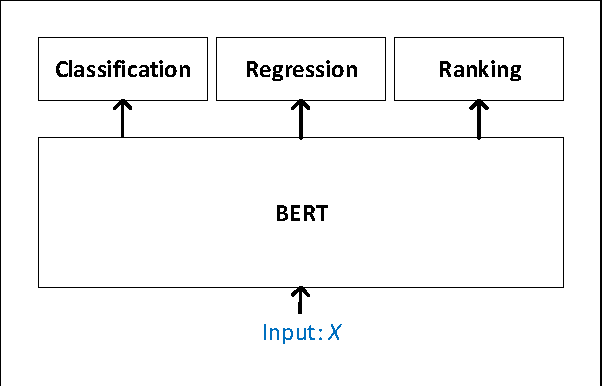
\includegraphics[scale=0.7]{mtl_model_v2}}
\caption{Model architecture version 2.}
\label{fig:mtl_model_v2} 
\end{figure}

\textbf{Task definition}

\textbf{Objective}

\textbf{Single classification}
\xiaodl{Need to cluster different tasks..}

\textbf{Sentence-pair classification}: given a pair of sentence, $(S_1, S_2)$, the model predicts a label indicating the relation of this pair of sentences: $P(C|S_1, S_2)$. For example, natural language inference is a typical instance of the sentence-pair classification task: a premise and a hypothesis are denoted by $S_1$ and $S_2$, respectively; the label, $C$, belongs one of three relations (\textit{contradiction}, \textit{neutral} and \textit{entailment}). 

\textbf{Regression}


\textbf{Pair-wise Ranking}
\begin{algorithm}[ht!]
 \SetAlgoLined
Initialize model parameters $\Theta$ randomly  \\
Set M \quad\textit{//the number of updates for the shared layer} \\
%\textit{Counter} = 0\\
 \For{$iteration$ in $0 ... \infty$}{
 	 %1. \textit{Counter} += 1\\
     1. Pick a task $t$ randomly \\
     2. Pick sample(s) from task $t$, i.e., \\
     \hspace{0.4cm}$(Q,C=\{0,1\})$ for classification \\
     \hspace{0.4cm}$(Q, D)$ for ranking\\
     3. Compute loss: $L(\Theta)$, i.e.,\\
     \hspace{0.4cm} the \textit{cross-entropy} for classification \\
     \hspace{0.4cm} the ranking loss for ranking\cite{learning-to-rank2005burges}\\

     4. Compute gradient: $\nabla(\Theta)$ \\
     5. Update model: $\Theta = \Theta - \epsilon \nabla(\Theta)$ \quad\textit{}
     % \eIf{Counter $<$ M}{
  	 %5. Update model: $\Theta = \Theta - \epsilon \nabla(\Theta)$ \quad\textit{//update both $\Theta^s$ and $\Theta^t$} \\
   %}{
   	% 6. Update model: $\Theta^t = \Theta^t - \epsilon \nabla(\Theta^t)$ 
  %}
 }
 \caption{\label{algo:mtdnn} Training a Multi-task model.}
 \algorithmfootnote{Note that $\Theta$ denotes the model parameters. \textcolor{red}{TODO: update alg based on task defination.}}
\end{algorithm}